\documentclass[]{article}



\usepackage[utf8]{inputenc}
\usepackage[T1]{fontenc}
\usepackage{mathptmx}
\usepackage[english]{babel}
\usepackage{graphicx}
\usepackage{amsmath}
\usepackage{amssymb}
\usepackage{amsfonts}
\usepackage{amsthm}
\usepackage{subcaption}

\usepackage{biblatex}
\addbibresource{./bibli.bib}

\usepackage{hyperref}
\graphicspath{ {plots/} }
\hypersetup{
	linktocpage=true,
	colorlinks=true,
	linkcolor=red,
	filecolor=magenta,      
	urlcolor=cyan,
	pdfpagemode=FullScreen,
	bookmarks=true,
	breaklinks=true
}

\urlstyle{same}
\newtheorem{thm}{Theorem}[section]
\newtheorem{cor}[thm]{Corollary}
\newtheorem{lem}[thm]{Lemma}
\newtheorem{definition}{Definition}[]

\newcommand{\norm}[1]{\left\lVert#1\right\rVert}
\newcommand{\Q}[0]{\textit{Q}}

\DeclareMathOperator*{\argmax}{argmax}
\DeclareMathOperator*{\argmin}{argmin}


%opening
\title{Approximation Final Work}
\author{Eldad Kronfeld}
\date{}

\begin{document}

\maketitle
\tableofcontents

\newpage
\section{Theoretical Question }
\subsection{Background}
\begin{definition}
	\label{definition1}
	Let $f$ be a continuous function on the interval $[a, b]$, and let $p$ be a polynomial approximation. An alternating set on $f, p$ is defined to be a sequence of points $x_{0}, ..., x_{n-1}$ such that:
	\begin{itemize}
	\item $a \leq x_0 <...<x_{n - 1}\leq b .$
	\item $f(x_i) - p(x_i) = (-1)^i E \text{ for } i=0,1,...,n-1.$ 
\end{itemize}
Where either $E=||f-p||$ or $E=-||f-p||$. The number $n$ is the length of the alternating set.
\end{definition}


\begin{thm}
	\label{thm1}
	Let $f \in C[a.b]$, and suppose that $p=p^{*}_{n}$ is the best approximation of $f$ out of $P_{n}[x]$, that is
	\begin{equation}
		||f-p||_{\infty} \le ||f-q||_{\infty} \text{ for all } q\in P_{n}[x] 
	\end{equation}
	Then, there is an alternating set for $f-p$ consisting of at least $n+2$  points.
	
\end{thm}
\subsection{Question}
Prove that the best approximation polynomial is unique using Theorem (\ref{thm1}). 
\begin{proof}
	The theorem is trivial if $f$ is polynomial of degree $\leq n$, so we assume that is not true. To show the uniqueness, suppose that both $p_n, q_n$ are polynomials of best approximation, and we will show that they are equal.
	Note that $\frac{(p_n + q_n)}{2}$ is also a polynomial of best approximation because:
	\begin{equation*}
		 \norm{f-\frac{(p_n + q_n)}{2}} = \norm{\frac{(f - p_n)}{2} \frac{(f - q_n)}{2}} \leq \frac{1}{2}\norm{f-p_n} + 
		 \frac{1}{2}\norm{f-q_n} = \pm E
	\end{equation*}
	Therefore, there are $n+2$ points at which:
	\begin{equation*}
		\frac{f-p_n}{2}+\frac{f-q_n}{2}=\pm E
	\end{equation*}
	At each of those alternating points both $f-p_n$ and $f-q_n$ are equal to $\pm E$ then we can say that at each of the $n+2$ points:
	\begin{equation*}
		(f(x_i) - p_n(x_i)) - (f(x_i)-q_n(x_i)) = 0 \text{ for each of the alternating point, }i=1..n+2
	\end{equation*}
	Since both $p_n,q_n$ are polynomials of degree$\leq$n then they must be identical, therefore $p_n$ is unique.
\end{proof}

\section{Practical question}
\subsection{Background}
\begin{definition}
	the \textbf{Chebyshev center}\cite{convexOptimization} of a bounded set $\textit{Q}\subseteq X$ with non-empty interior is the center of the smallest ball that encloses the entire of the set $\Q$,and the radius is:
	\begin{equation*}
		r=\inf\{\sup\{\norm{x-y}:x\in\Q\}:y\in X\}
	\end{equation*}
\end{definition}
The Chebyshev center is described as the solution to the following optimization problem:
\begin{equation}
	\label{OP1}
	\begin{aligned}
		\min_{\hat{x},r} \quad &r \\
		\text{s.t.}\quad &\norm{\hat{x} - x} \leq r \text{ for all }x\in\Q \\
		\quad & r\geq 0
	\end{aligned}
\end{equation}
The optimization problem states that the radius r is the target function we would like to minimize which is subjected to two types of constraints:
\begin{itemize}
	\item All the points of $\Q$ are inside.
	\item $r$ needs to be non-negative, as it is the radius of the ball.
\end{itemize}
It could also be described as the solution to the min-max problem
\begin{equation}
	\label{OP2}
	\argmin_{\hat{x}} \max_{x\in\Q} \space \norm{x-\hat{x}}
\end{equation}
Which translate to the minimization of the distance of the furthest point from the center. Both of the optimization problems correspond to the first definition of Chebyshev centers.\\
\textbf{Note:} other books and papers\cite{ParametricOptimization} define the Chebyshev centers differently which is not equivalent to the definition (\ref{definition1}).
\begin{definition}
	\label{definition2}
	The \textbf{Chebyshev center} of a bounded set $\Q\subseteq X$ with non-empty interior is the center of the largest ball inscribed in $\Q$, and the center is:
	\begin{equation}	
		\hat{x}=\argmax_{x\in X}\space d(x,\Q) = \argmax_{x\in X} \space \min_{y\in \Q} \norm{\hat{x} - x}
	\end{equation}
\end{definition}
The difference between the two definitions (\ref{definition1}) and (\ref{definition2}) is that definition (\ref{definition1}) denotes the center that encloses the set $\Q$ like in figure (\ref{exp1}). However the second definition (\ref{definition2}) states that the ball should be enclosed by the set $\Q$, like in figure (\ref{exp2}) and not the other way around.

\paragraph{Chebyshev center as a Linear programming problem \\}
In contrast to the optimization problems above (\ref{OP1}, \ref{OP2}) the definition used in order to construct the linear problem is definition (\ref{definition2}). In order to solve the problem, the set $\Q$ must be represented as an intersection of finitely many half-spaces. The intersection, if non-empty, creates a convex polytope, which is a geometrical object with flat faces created by the intersection of half-spaces as can be seen in figure \ref{Fig:polytope}.

\begin{figure}[!h]
	
	\begin{subfigure}{0.5\textwidth}
		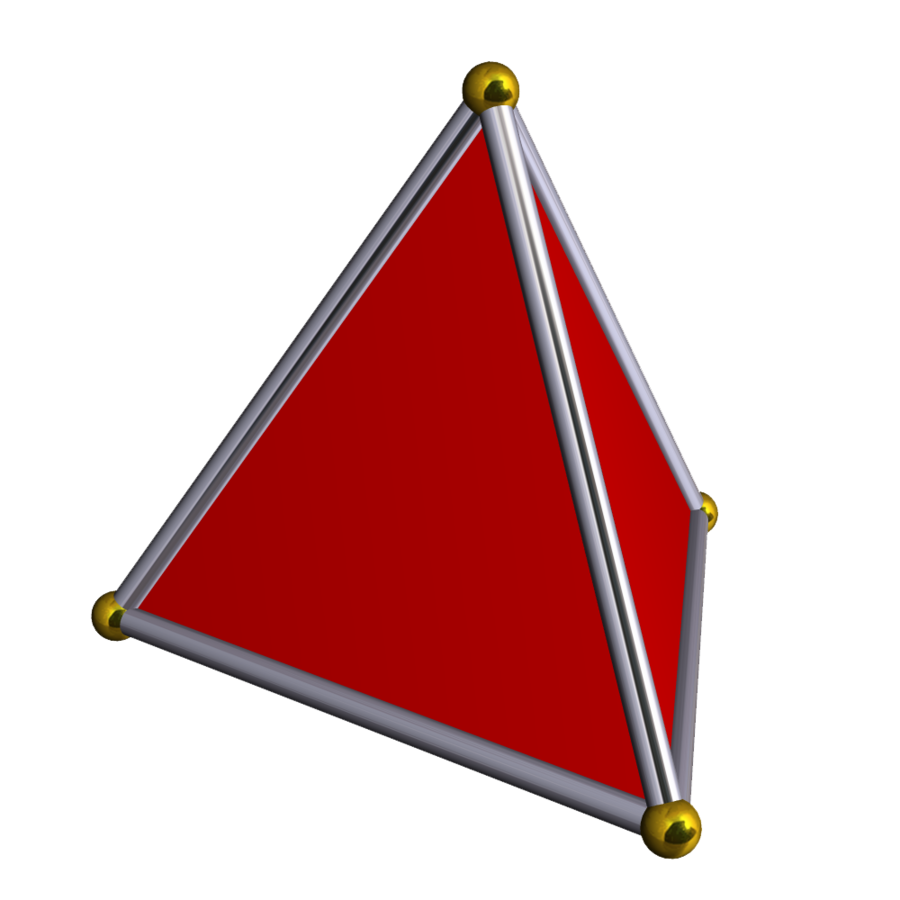
\includegraphics[width=1\linewidth,height=\textwidth]{Tetrahedron}
		\caption{tetrahedron}
	\end{subfigure}
	\begin{subfigure}{0.5\textwidth}
		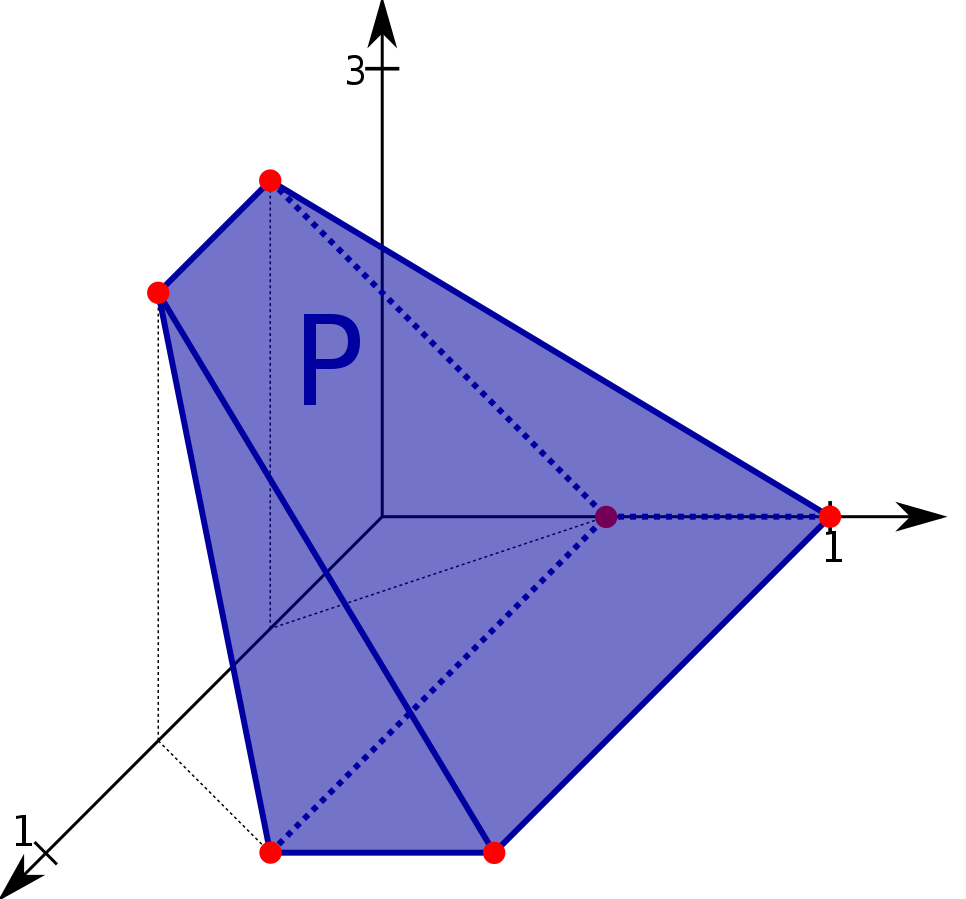
\includegraphics[width=1\linewidth,height=\textwidth]{3dpoly}
		\caption{3-dimensional convex polytope}
	\end{subfigure}
	\caption{Two examples for convex polytopes.}
	\label{Fig:polytope}
\end{figure}

The Chebyshev center could be found by solving the following problem:
\[\Q = \{ x\in \Re^n : Ax\leq b\}\]
\begin{equation}
	\label{LP}
	\begin{aligned}
		\min_{\hat{x},r} \quad &r \\
		\text{s.t.}\quad & a_i \hat{x} + \norm{a_i}r \leq b_i \text{, for every half-space of } \Q \\
		\quad & r\geq 0
	\end{aligned}
\end{equation}

The optimization's target function is the same as before, but because the second definition (\ref{definition2}) is used in this formulation, then instead of minimizing the radius of the ball into the set $\Q$, we maximize the radius of the ball inside of it, while the constants require us that the ball and it's sphere should be inside of the convex polytope.
 
\subsection{Experiments}

The conducted Experiments included two steps: randomizing data points in the 2d plane, then constructing and solving the optimization problem in order to find the Chebyshev center and it's radius.
Randomizing the data was relatively simple process, I decided to randomize 20 points in the 2d plane as a proof of concept. The coordinates for each of the points was in the range of $[-25,25]$ in order to spread them in the 2d plane, then I calculated the convex hull of the points, in order to create a set that fits both definition (\ref{definition1}) and definition (\ref{definition2}).

\subsubsection{Experiment 1 - calculating the bounding circle of the convex hull}

The experiments took the the points (including the boundaries of the convex hull) and solved the problem defined in (\ref{OP1}) in order to find the enclosing circle of the set of points.

\paragraph{The non-linear solver\\}
To solve the problem I used the function \textit{fmincon} in matlab, which takes the objective function and the non-linear constraints and solves the problem using an algorithm called "\textbf{interior point}". The algorithm solves a sequence of approximated minimization problems that convert the inequalities into equality constraints because they are easier to solve (the exact technique that is used is called barrier function \cite{barrier}). Then the algorithm uses one of two main types of steps at each iteration:
\begin{itemize}
	\item A direction step, which attempts to solve the KKT equation via linear approximation, this is also called Newton step.
	\item A CG (conjugate gradient) step, using trust region.
\end{itemize}
At first the algorithm attempts to take a direction step, if it cannot The algorithm attempts a CG step. \newline

The solver provided us a solution $(x,y,r)$ where $x,y$ are the coordinates of the Chebyshev center and $r$ is the radius of the circle that encompasses the set of points. As we can see in figure (\ref{exp1}) the solution encompasses both the points and the convex hull, while the area covered by the hull is $A_{hull}= 1266$ the area covered by the circle is $A_{circle} = 2441$ which is significantly larger then the actual convex hull.

\begin{figure}[!h]
	\centering
	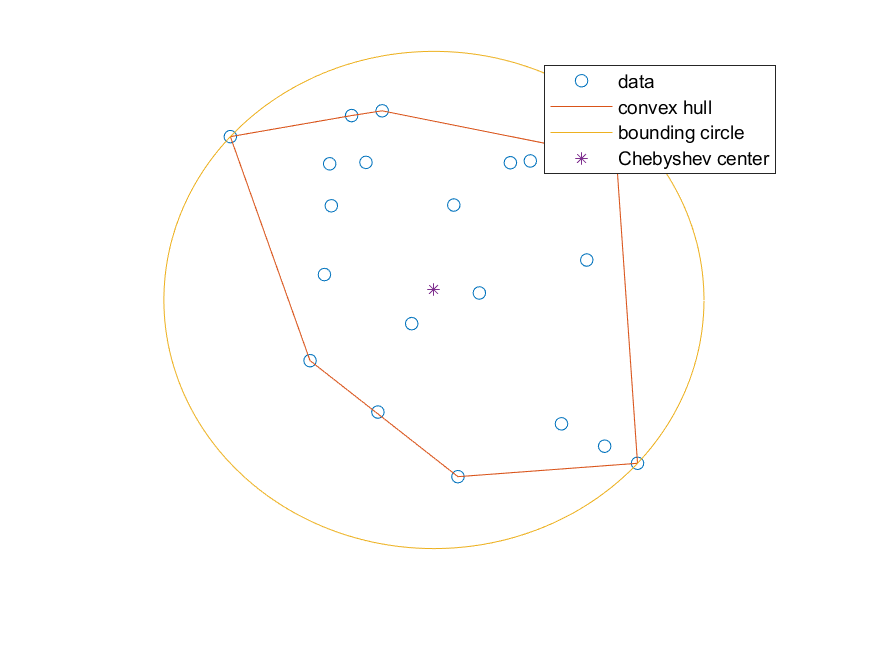
\includegraphics[width=\textwidth]{bounding}
	\caption{The results for the first experiment on the plane with the randomized data}
	\label{exp1}
\end{figure}

\subsubsection{Experiment 2 - calculating the inscribed circle on intersection of half-spaces}

In order to find the inscribed ball as defined in (\ref{definition2}) the set $\Q$ needs to be a an intersection of half-spaces. Because of that fact I chose to create the data as points and calculate the hull as it is easy to look at the convex hull as the intersection of the half-spaces defined by the boundaries of it. In order to figure the inequalities of the half-spaces I used the formula for a straight line \[(x_2-x_1)y - (y_2-y_1)x = (x_2-x_1)y_1 - (y_2-y_1)x_1\] Then I determined the sign of the inequality using a point inside of the convex hull (the average of the vertices in the boundary).\newline

After calculating the inequalities and producing the system $Ax \leq b$ that defines the convex hull, I created the constraints and target function as defined in (\ref{LP}). The results can be shown in figure (\ref{exp2}), in this experiment the area of the circle was $A_{circle} = 898.4991$ and as before the area of the convex hull was $A_{hull}= 1266$. 


\begin{figure}[!h]
	\centering
	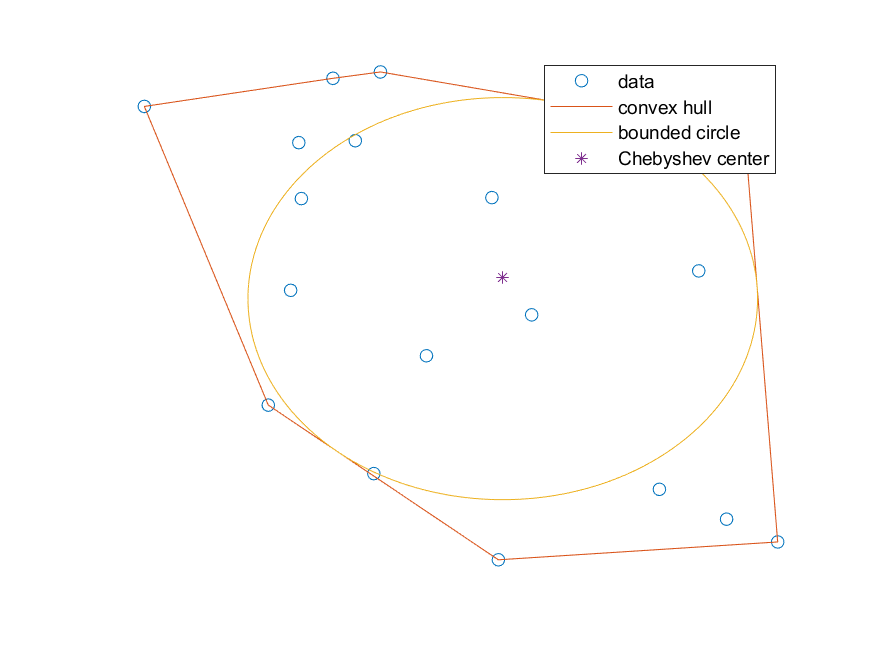
\includegraphics[width=\textwidth]{bounded}
	\caption{The results for the second experiment on the plane with the randomized data}
	\label{exp2}
\end{figure}

\subsubsection{Experimental conclusion}
Even though the definitions are not equivalent, they both can be handy in different scenarios, when $100\%$ is mandatory even at the expense of fitting a bigger ball, then the ball in experiment 1 would be the one chosen, however in cases where bigger coverage may cost more money or include outlier data-points then the second ball from experiment 2 would be the better one.
In figure (\ref{both}) we can see how much bigger is the bounding circle in comparison to the actual set and the inscribed circle, actually the bounding circle is $2.7$ times larger then the inscribed ball and around $2$ times larger then the area inside of the convex hull.

\begin{figure}[!h]
	\centering
	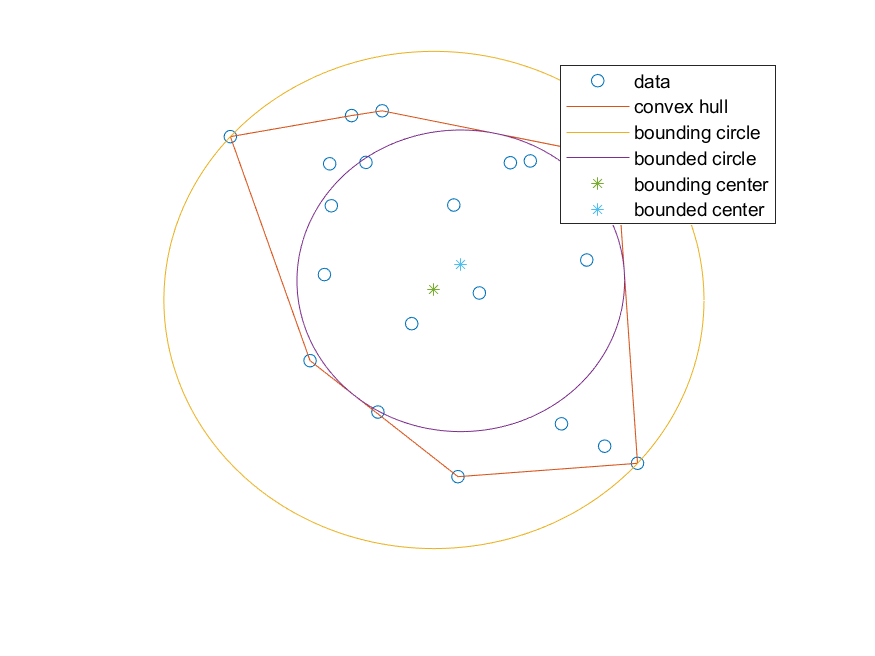
\includegraphics[width=\textwidth]{both}
	\caption{The results of both of the experiments together}
	\label{both}
\end{figure}

\subsection{Practical use}

Chebyshev centers have many practical uses, I will now point some of those out:
\begin{enumerate}
	\item \underline{\textbf{Parameter estimation}}\cite{doi:10.1137/060656784}\cite{4471880}- The Chebyshev center approach tries to find an estimator $\hat{x}$ for given points in feasibility set $\Q$ such that $\hat{x}$ minimizes the worst possible estimation error for the points in the set $\Q$.
	\item \underline{\textbf{Logistic planning}}- in cases where we want to place a warehouse or a logistics center that covers a region, but we want to minimize the longest distance between the logistics center and the furthest point in the region.
	\item \underline{\textbf{wireless networking}}- in order to cover an area the best we need to place an antenna in a spot where it can reach most if not all of a certain region.
\end{enumerate}

\section{Conclusion}
To conclude, Chebyshev center gives us a unique geometrical solution to the bounding sphere and coverage problem. It is also used in computer graphics, Machine learning and many other areas where estimation, grouping or simply trying to fill/encompass a region.



\printbibliography[
heading=bibintoc,
title={References}
]

\end{document}
